%%%%%%%%%%%%%%%%%%%%%%%%%%%%%%%%%%%%%%%%%
% Beamer Presentation
% LaTeX Template
% Version 1.0 (10/11/12)
%
% This template has been downloaded from:
% http://www.LaTeXTemplates.com
%
% License:
% CC BY-NC-SA 3.0 (http://creativecommons.org/licenses/by-nc-sa/3.0/)
%
%%%%%%%%%%%%%%%%%%%%%%%%%%%%%%%%%%%%%%%%%

%----------------------------------------------------------------------------------------
%	PACKAGES AND THEMES
%----------------------------------------------------------------------------------------

\documentclass[10pt]{beamer}

\mode<presentation> {

% The Beamer class comes with a number of default slide themes
% which change the colors and layouts of slides. Below this is a list
% of all the themes, uncomment each in turn to see what they look like.

\renewcommand{\familydefault}{\rmdefault}

\graphicspath{ {./figures/} }
\usepackage{graphicx} % Allows including images
\usepackage{booktabs} % Allows the use of \toprule, \midrule and \bottomrule in tables
\usepackage{tikz} % Allows the use of \toprule, \midrule and \bottomrule in tables
\usepackage{hyperref}
\usepackage[printwatermark]{xwatermark}

\usetheme{default}
% \usetheme{AnnArbor}
% \usetheme{Antibes}
% \usetheme{Bergen}
% \usetheme{Berkeley}
% \usetheme{Berlin}
% \usetheme{Boadilla}
% \usetheme{CambridgeUS}
% \usetheme{Copenhagen}
% \usetheme{Darmstadt}
% \usetheme{Dresden}
% \usetheme{Frankfurt}
% \usetheme{Goettingen}
% \usetheme{Hannover}
% \usetheme{Ilmenau}
% \usetheme{JuanLesPins}
% \usetheme{Luebeck}
% \usetheme{Madrid}
% \usetheme{Malmoe}
% \usetheme{Marburg}
% \usetheme{Montpellier}
% \usetheme{PaloAlto}
% \usetheme{Pittsburgh}
% \usetheme{Rochester}
% \usetheme{Singapore}
% \usetheme{Szeged}
% \usetheme{Warsaw}

% As well as themes, the Beamer class has a number of color themes
% for any slide theme. Uncomment each of these in turn to see how it
% changes the colors of your current slide theme.

% \usecolortheme{albatross}
\usecolortheme{beaver}
% \usecolortheme{beetle}
% \usecolortheme{crane}
% \usecolortheme{dolphin}
% \usecolortheme{dove}
% \usecolortheme{fly}
% \usecolortheme{lily}
% \usecolortheme{orchid}
% \usecolortheme{rose}
% \usecolortheme{seagull}
% \usecolortheme{seahorse}
% \usecolortheme{whale}
% \usecolortheme{wolverine}

%\setbeamertemplate{footline} % To remove the footer line in all slides uncomment this line
\setbeamertemplate{footline}[page number] % To replace the footer line in all slides with a simple slide count uncomment this line

\setbeamertemplate{navigation symbols}{} % To remove the navigation symbols from the bottom of all slides uncomment this line

% \setbeamertemplate{background}{
%     \tikz[overlay,remember picture]\node[opacity=0.4]at (current page.center){
%         \includegraphics[width=2cm]{iot_analytics_logo.jpg}
%         }}

}

%----------------------------------------------------------------------------------------
%	TITLE PAGE
%----------------------------------------------------------------------------------------

\title[What Phone do People Like?]{Phone Sentiment Analysis with Web Crawl Data} % The short title appears at the bottom of every slide, the full title is only on the title page

\author{Tuomo Kareoja} % Your name
\institute[Alert! Analytics] % Your institution as it will appear on the bottom of every slide, may be shorthand to save space
{
Alert! Analytics \\ % Your institution for the title page
\medskip
}
\date{\today} % Date, can be changed to a custom date

\begin{document}

\begin{frame}
\titlepage % Print the title page as the first slide
\end{frame}

\begin{frame}
\frametitle{Agenda} % Table of contents slide, comment this block out to remove it
\tableofcontents % Throughout your presentation, if you choose to use \section{} and \subsection{} commands, these will automatically be printed on this slide as an overview of your presentation
\end{frame}

%----------------------------------------------------------------------------------------
%	PRESENTATION SLIDES
%----------------------------------------------------------------------------------------

%------------------------------------------------
\section{Summary of Findings}
%------------------------------------------------

\begin{frame}
\frametitle{

}
\LARGE{\centerline{Summary of Findings}}
\end{frame}

%------------------------------------------------
\subsection{People Like iPhone More}
%------------------------------------------------

\begin{frame}
\frametitle{People Like iPhone More}

\begin{itemize}
    \item When the sites actually mention the phones, iPhone sentiment is much more positive
\end{itemize}

{
    \centering
    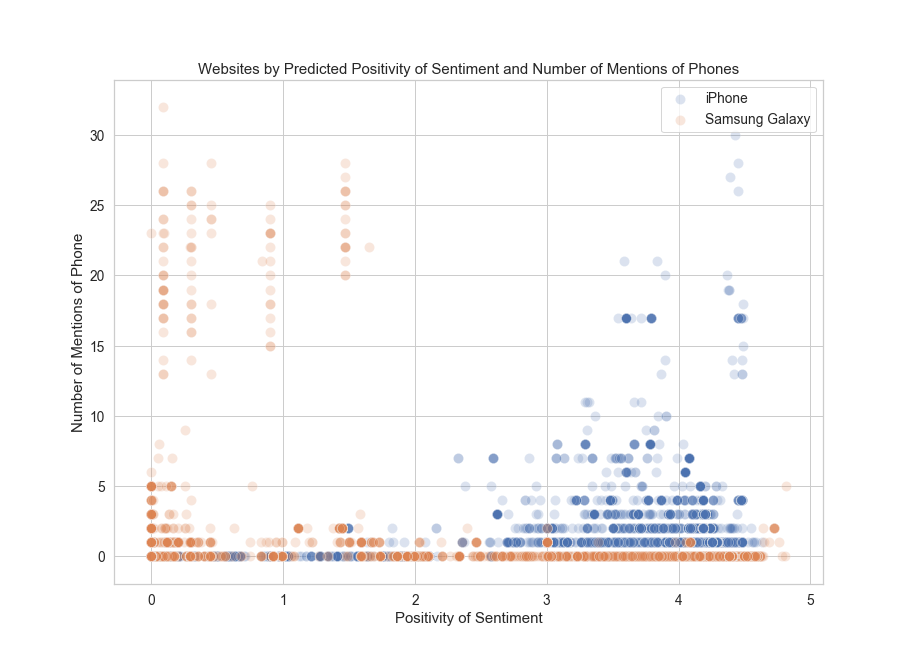
\includegraphics[width=\textwidth,height=\textheight,keepaspectratio]{sentiment_comparison_predictions.png}
    \par
}

\end{frame}

%------------------------------------------------
\subsection{\ldots but the Training Data is Sketchy}
%------------------------------------------------

\begin{frame}
\frametitle{\ldots but the Training Data is Sketchy}

\begin{itemize}
    \item Sentiment labels for Samsung Galaxy might be derived from iPhone (somebody was lazy and cheated!)
\end{itemize}

{
    \centering
    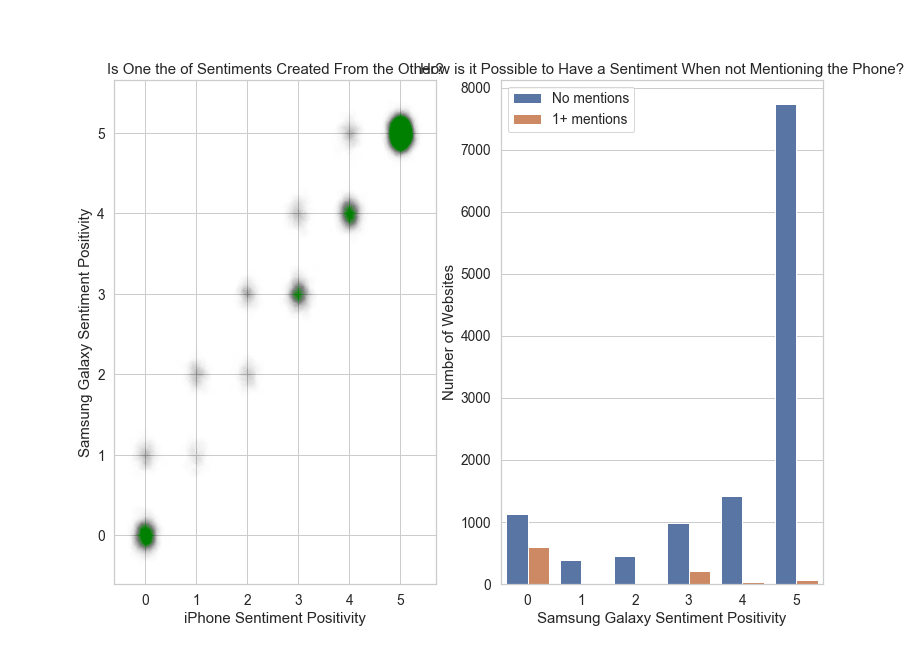
\includegraphics[width=\textwidth,height=\textheight,keepaspectratio]{training_data_problems.png}
    \par
}

\end{frame}

%------------------------------------------------
\subsection{\ldots and the Websites Mentioning iPhone are Weird}
%------------------------------------------------

\begin{frame}
\frametitle{\ldots and the Websites Mentioning iPhone are Weird}

\begin{itemize}
    \item Danhostel is a danish hotel chain
    \item http://brazoriacountytexas.tk/ is maze for web crawling without any content
\end{itemize}

{
    \centering
    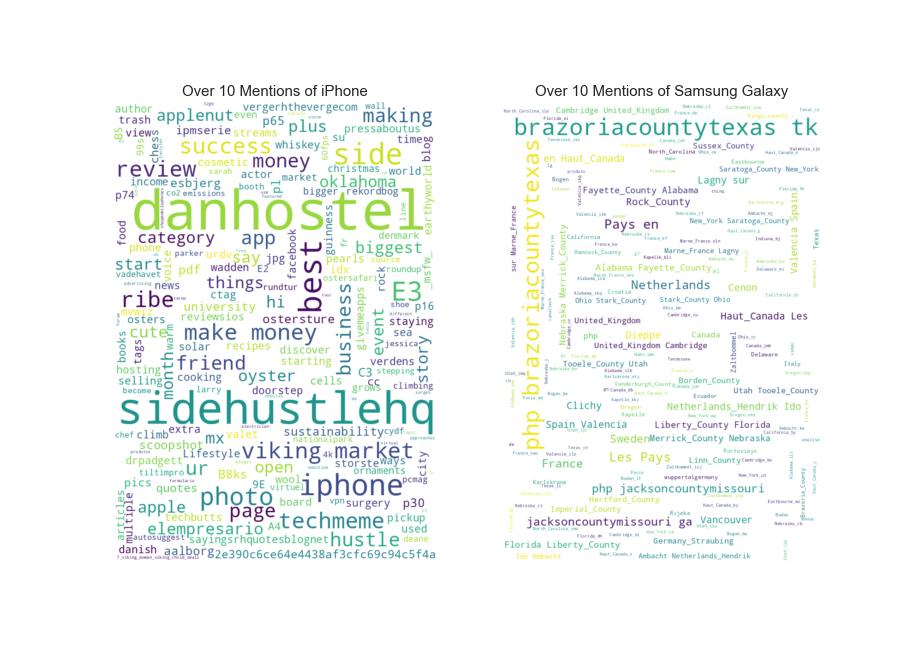
\includegraphics[width=\textwidth,height=\textheight,keepaspectratio]{wordclouds_for_sites_with_lots_of_mentions.png}
    \par
}


\end{frame}

%------------------------------------------------
\section{What We Did?}
%------------------------------------------------

\begin{frame}
\frametitle{

}
\LARGE{\centerline{What We Did?}}
\end{frame}

%------------------------------------------------
\subsection{Crawl Websites and Count Word Instances}
%------------------------------------------------

\begin{frame}
\frametitle{Count Instances of Word and Word Combinations from Websites}

\begin{enumerate}
    \item Create scripts that count instances of words related to the the two phones in text files
    \item Apply the scripts to a large number of websites taken from Common Crawl (cloud computing very useful here)
    \item Manually label part of the dataset for the sentiment towards the phones
    \item Predict the manually labeled sentiments from the number of word instances
\end{enumerate}


\end{frame}

%------------------------------------------------
\subsection{Modelling}
%------------------------------------------------

\begin{frame}
\frametitle{Modelling}

\begin{itemize}
    \item Random Forest model perform accurately and is very stabile
\end{itemize}

{
    \centering
    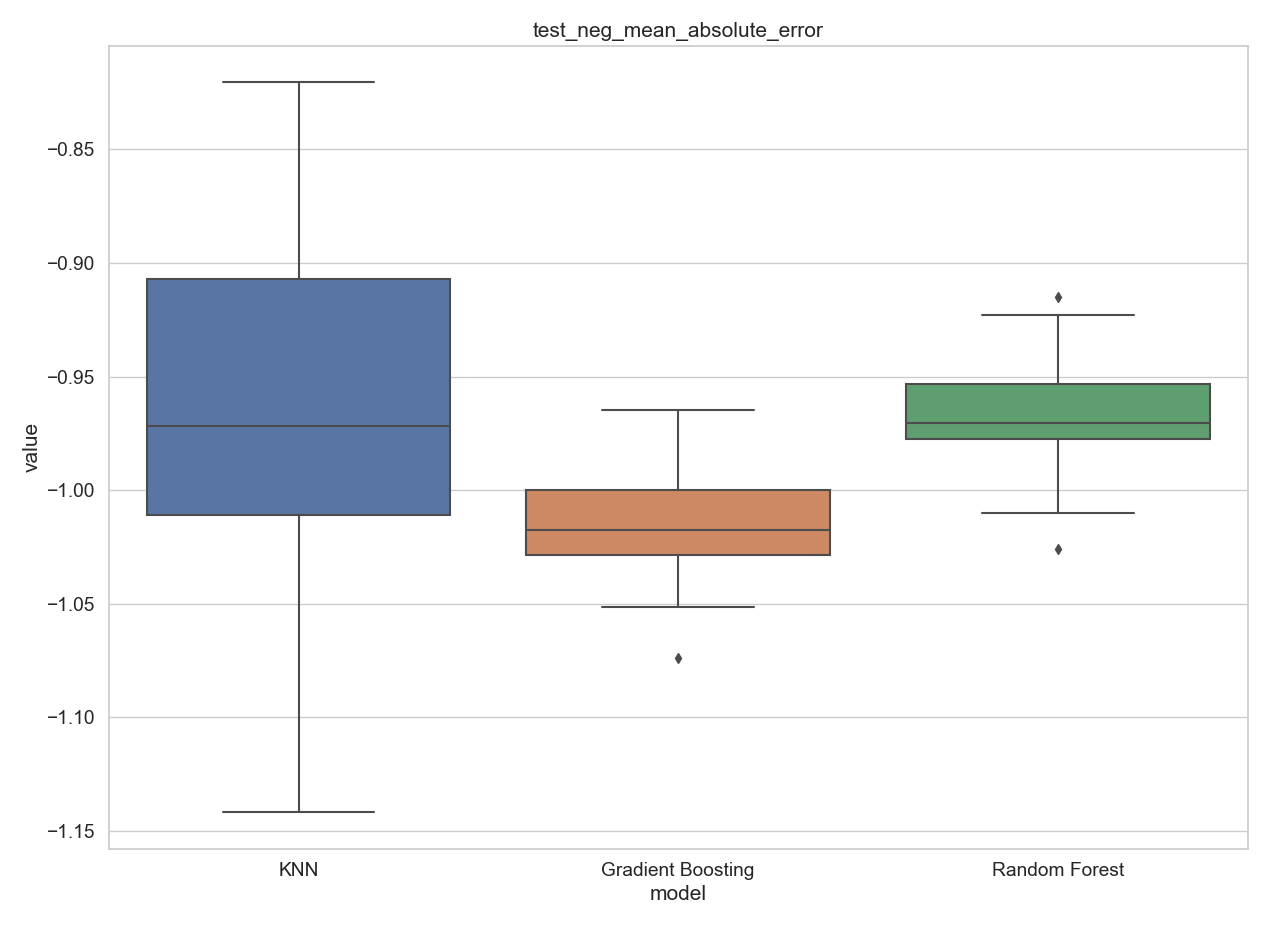
\includegraphics[width=\textwidth,height=0.8\textheight,keepaspectratio]{model_comparison_iphone_test_neg_mean_absolute_error.png}
    \par
}

\end{frame}

%------------------------------------------------
\section{What To Do Better Next Time?}
%------------------------------------------------

\begin{frame}
\frametitle{

}
\LARGE{\centerline{What To Do Better Next Time?}}
\end{frame}


%------------------------------------------------
\subsection{Better Training Data}
%------------------------------------------------

\begin{frame}
\frametitle{Better Training Data}

\begin{enumerate}
    \item Better Documentation
    \begin{itemize}
        \item Was the labeling really done by hand and if so, what were
        the guidelines for evaluation?
        \item If done programmatically, where is the code?
    \end{itemize}
    \item Check for Errors
    \begin{itemize}
        \item Why are the sentiment almost identical for the two phones?
        \item How can sites that don't mention phones have sentiments about them?
    \end{itemize}
\end{enumerate}

\end{frame}

%------------------------------------------------
\subsection{Aggressive Limitations on What Sites to Crawl}
%------------------------------------------------

\begin{frame}
\frametitle{Aggressive Limitations on What Sites to Crawl}

\begin{enumerate}
    \item Think first what kind of sites do we want to include
    \begin{itemize}
        \item Reviews and news probably easy to find
        \item Forums are hard to interpret
        \item Beware of clickbait and ads
    \end{itemize}
    \item Test that crawling really finds these sites
    \begin{itemize}
        \item Wordclouds of the url
        \item Manually visiting the sites
    \end{itemize}
\end{enumerate}

\end{frame}

%------------------------------------------------
\section{Conclusions}
%------------------------------------------------

\begin{frame}
\frametitle{Conclusions}

\begin{enumerate}
    \item Don't trust the current findings. Make the decision by other means
    \item More carefully documented labeling in the future
    \item Web crawling should be more targeted
\end{enumerate}

\end{frame}

\begin{frame}
\frametitle{The End}

\LARGE{\centerline{Questions?}}

\end{frame}

%----------------------------------------------------------------------------------------

\end{document}
